%----------------------------------------------------------------------------------------
% Modelos Ocultos de Márkov
%----------------------------------------------------------------------------------------

Esta práctica introduce el concepto de Modelo Oculto de Márkov, así como sus aplicaciones en el aprendizaje supervisado de cadenas, en donde se implementará el algoritmo de Viterbi.

\section{Objetivo}

Que el alumno conozca el concepto de Modelo Oculto de Márkov, su forma de representarlos, así como sus aplicaciones. Que sea capaz de aplicar los Modelos Ocultos de Márkov a problemas de etiquetado de secuencias de forma óptima por medio del algoritmo de Viterbi.


\section{Introducción}

Los Modelos Ocultos de Márkov a los que nos referiremos como HMM (por sus siglas en inglés \emph{Hidden Markov Models}) son un modelo gráfico \emph{generativo}.  Esto es, son capaces de aprender un modelo de la distribución de probabilidad subyacente a los datos de entrenamiento y utilizarlo para generar nuevos datos con características semejantes.  Además, generalizan el modelo de Bayes Ingenuo e incorporan el concepto de procesos de Márkov en su estructura, es decir, que asumimos un sistema dinámico en el que el estado al tiempo $t$ depende sólo del estado al tiempo $t-1$.

En el clasificador de Bayes Ingenuo se busca estimar una probabilidad conjunta de una serie de observaciones, determinadas por un vector, $x$ y las clases $y$. En el modelo de Bayes Ingenuo se busca estimar la clase $\hat{y}$ que cumpla:

$$ \hat{y} = \arg\max_y P(y,x) = \arg\max_y p(x|y)$$

Es decir, aquella clase $\hat{y}$ que maximice la probabilidad de haber observado a $x$.  Si $x$ es un vector con $n$ elementos independientes, la probabilidad condicionada a $y$ puede expresarse como $P(x|y) = \prod_{i=1}^n P(x_i | y)$. El modelo de Bayes Ingenuo es de gran utilidad para clasificar un vector de rasgos dentro de una clase o categoría que lo represente. Sin embargo, hay problemas, como el etiquetado de cadenas del lenguaje natural, donde lo que se busca es pasar de una cadena a otra. Por ejemplo, si en una cadena del lenguaje natural como: ``yo salto el salto'', queremos identificar los tipos de palabras (nombre común, verbo, preposición, pronombre, etc.), no basta con clasificar cada palabra según su clase más probable pues, como se puede observar en este ejemplo, la etiqueta depende del contexto. Así, la palabra ``salto'' es en el primer caso un verbo (ya que es precedido por un pronombre) y en el segundo un nombre común (antecedido por el artículo).

\begin{figure}
 \centering
 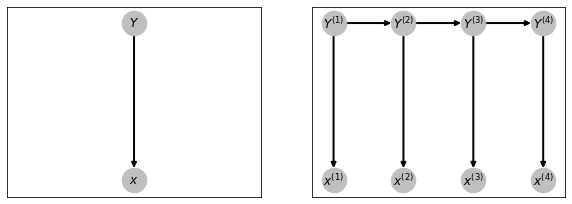
\includegraphics[width=1.0\textwidth]{hmm/hmmBayes}
 \caption{Comparación entre la gráfica del modelo de Bayes Ingenuo y la gráfica de un Modelo Oculto de Márkov.}\label{Fig:BayesMárkov}
\end{figure}

Los HMMs son una solución a este tipo de problemas. Podemos pensar a un HMM como un modelo de Bayes Ingenuo dinámico, donde las clases o categorías conforman un proceso de Márkov. En la \fref{Fig:BayesMárkov} se puede observar la comparación entre una gráfica del modelo de Bayes Ingenuo (a la izquierda) y el modelo oculto de Márkov (a la derecha). El HMM genera transiciones entre las cadenas de salida, para así poder estimar la pertinencia de una categoría en referencia no sólo a una observación, sino a las categorías previas de la cadena. En términos generales, definimos una HMM como sigue:


\begin{definition}[Modelo Oculto de Márkov]
  Un \emph{Modelo Oculto de Márkov} o HMM es un modelo bayesiano definido como una 5-tupla $HMM = (X, Y, A, \Pi, B)$ cuyos elementos son:

\begin{itemize}
    \item $X$ es un conjunto de \emph{observables} que dependen de $Y$.
    \item  $Y$ es un conjunto de \emph{emisiones} que definen un proceso de Márkov.
    \item $A$ es la matriz de transiciones y $\Pi$ es un vector de probabilidades iniciales; ambos definen el proceso de Márkov sobre $Y$.
    \item $B$ es una matriz de probabilidades de observaciones, que contiene las probabilidades de las observaciones condicionadas a las emisiones.
  \end{itemize}
\end{definition}

Para obtener la cadena de emisiones $\hat{y_1}, \hat{y_2}, ... , \hat{y_n}$ más óptima, que etiquete a la cadena de entrada $\hat{x_1}, \hat{x_2}, ... , \hat{x_n}$, se debe optimizar la probabilidad conjunta:

\begin{align} 
    \small
    \hat{y_1}, \hat{y_2}, ... , \hat{y_n} &= \arg\max_{y_1,...,y_n} P(Y^{(1)}=y_1, Y^{(2)}=y_2,...,Y^{(n)}=y_n, x^{(1)}, x^{(2)}, x^{(n)}) \nonumber \\
    &= \arg\max_{y_1,...,y_n} \prod_{t=1}^n P(Y^{(t)}=y_t | Y^{(t-1)}=y_{t-1}) P(x^{(t)}|Y^{(t)}=y_t) \label{eq:HMM}
\end{align}

Con la convención de que $P(Y^{(1)}=y_1) :=P(Y^{(1)}=y_1 | Y^{(0)})$ es la probabilidad inicial del proceso de Márkov en $Y$. Esto establece los HMM y da forma al problema que buscamos resolver.
    




\subsection{Estimación del modelo}

Un HMM puede considerarse un modelo de aprendizaje; es decir, un modelo en que se deben aprender ciertos parámetros a partir de un conjunto de datos. Con estos datos, se deben obtener los valores que pueden tomar $Y$ y $X$, así como las probabilidades de transición ($A$), iniciales ($\Pi$) y de observaciones ($B$). Al proceso de obtener los parámetros del modelo se le conocerá como el \emph{entrenamiento del modelo}.

Tomemos un caso en donde queremos obtener cadenas en un alfabeto $Y = \{a,b,c\}$ a partir de un alfabeto binario $X = \{0,1\}$. Tenemos entonces que estimar un modelo para el proceso de Márkov en $Y$ determinado por las transiciones, la probabilidad de que se pase de un símbolo en $Y$ a otro, y las probabilidades iniciales. Pero además, tenemos que estimar las probabilidades de observaciones, esto es, la probabilidad de observar un símbolo binario asociado a un símbolo del alfabeto $\{a,b,c\}$.

Podemos asumir que las probabilidades de transición en $A$ son las siguientes:

\begin{center}
 \begin{tabular}{l|ccc}
  \multicolumn{4}{c}{$P(Y^{(t)}|Y^{(t-1)})$} \\ \hline
  $Y^{(t)}$ \textbackslash $Y^{(t-1)}$          & a & b & c \\ \hline
  a &    0.1   &    0.7  & 0.6 \\
  b   &    0.5   &    0  & 0.2 \\
  c    &    0.4    &   0.3  & 0.2
 \end{tabular}
 \end{center}

Y consideremos los siguientes iniciales $\Pi$:

\begin{center}
 \begin{tabular}{l|c}
  \multicolumn{1}{c|}{$y_0$}   &  $P(Y^{(0)})$ \\ \hline
  a &    0.4 \\
  b   &    0.3 \\
  b    &    0.3
 \end{tabular}
 \end{center}

Como se puede observar, el HMM define un proceso de Márkov sobre $Y$, pero además integra un modelo de predicción; consideremos entonces las probabilidades de observaciones en $B$ dadas como:

\begin{center}
 \begin{tabular}{l|ccc}
  \multicolumn{4}{c}{$P(x^{(t)}|Y^{(t)})$} \\ \hline
  $x^{(t)}$ \textbackslash $Y^{(t)}$   & a & b & c \\ \hline
  0 &    0.6   &    0.3  & 0.2 \\
  1   &    0.4   &    0.7  & 0.8 
 \end{tabular}
 \end{center}

 Esta matriz de observaciones guarda similitudes con el modelo de Bayes Ingenuo, pues se puede decir que determina las probabilidades condicionadas a su clase. En la forma gráfica del modelo, expuesta en la Figura~\ref{Fig:BayesMárkov} (derecha), las probabilidades de transición en $A$ determinan las aristas horizontales que van de una variable $Y^{(t)}$ hacia la siguiente, mientras que la matriz $B$ determina las aristas verticales entre los elementos $Y^{(t)}$ y $x^{(t)}$.

 Si bien el modelo gráfico que define a las HMMs está determinado por la gráfica secuencia de la Figura~\ref{Fig:BayesMárkov}, es común representar a los parámetros del modelo en una gráfica, que se define como sigue:

 \begin{enumerate}
     \item Se tiene un nodo raíz que indica el comienzo.
     \item Desde el nodo raíz se generan aristas hacia los símbolos en $Y$ con las probabilidades iniciales.
     \item Se generan aristas entre todos los símbolos en $Y$ que representan las probabilidades de transición.
     \item De los símbolos en $Y$ se generan aristas hacia los símbolos en $X$ con las probabilidades de observación.
 \end{enumerate}

 Por ejemplo, del modelo anterior se obtiene la gráfica de la Figura~\ref{Fig:hmmGraph}, la cual resume de manera visual el modelo $HMM = (X,Y, A,\Pi, B)$. Sin embargo, cuando se tienen muchos símbolos este tipo de gráficas se hacen complejas y no es conveniente realizarlas.


\begin{figure}
 \centering
 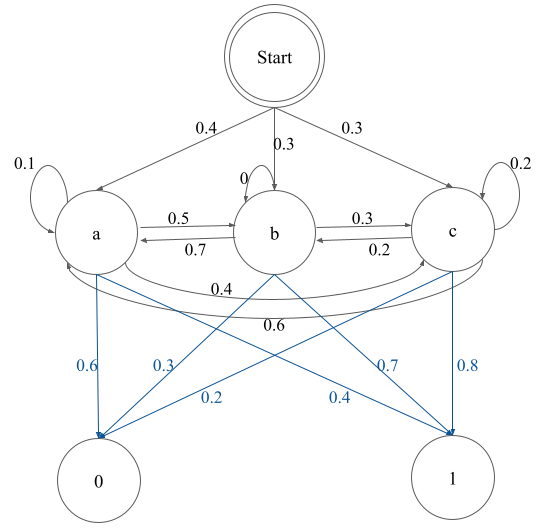
\includegraphics[scale=0.5]{hmm/hmmGraph.png}
 \caption{Gráfica que representa los parámetros del HMM.}\label{Fig:hmmGraph}
\end{figure}





\subsection{Etiquetado con HMMs}

Para realizar el etiquetado de una cadena de entrada $x^{(1)}, x^{(2)},...,x^{(n)}$ dado un HMM, se requiere encontrar la cadena que solucione el problema de optimización de la Ecuación~\ref{eq:HMM}. Sin embargo, como se está computando un máximo, se deben explorar todos los símbolos posibles $y_t$ para cada uno de los estados de la cadena. Así, por ejemplo, si $|Y| = M$ es el número de símbolos de emisión, se tendrá que calcular $M$ probabilidades para una cadena de longitud 1. Para una cadena de longitud 2, el primer símbolo de entrada podrá tomar $M$ valores, y el segundo también podrá tomar estos $M$ valores, por lo que se tendrán que calcular $M^2$ combinaciones, para de ahí poder tomar la que haya dado la probabilidad más alta. En general, encontrar el argumento que maximiza la probabilidad sobre las cadenas de emisión tiene una complejidad de $O(M^n)$.

En problemas reales, como etiquetado del lenguaje natural, donde se cuenta con cadenas de varios cientos de símbolos, y cadenas que pueden tener la extensión de un documento, el cálculo de estas probabilidades se vuelve intratable. En la Figura~\ref{Fig:Trellis} se muestra un diagrama, conocido como diagrama de Trellis, que muestra los posibles formas de etiquetar la cadena ``yo salto el salto de altura'' con cinco símbolos de emisión.\footnote{Los símbolos corresponden a las etiquetas $DA=$Determinante Artículo, $NC=$Nombre Común, $PP=$Preposición, $DP=$Determinante Pronombre y $V=$Verbo.} Partiendo de cualquier símbolo de inicio se puede tomar cualquier camino, lo que genera un total de $5^6=15 625$ posibles caminos, o formas de etiquetar la cadena.


\begin{figure}
    \centering
    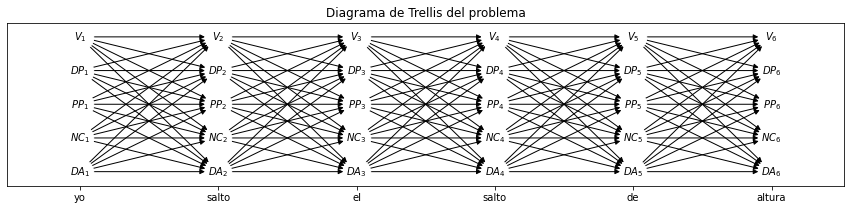
\includegraphics[width=1\textwidth]{hmm/trellis}
    \caption{Diagrama de Trellis que muestra todos los caminos posibles para etiquetar una cadena de longitud 6 con 5 emisiones.}
    \label{Fig:Trellis}
\end{figure}

\subsection{Algoritmo de Viterbi}

Para solventar la complejidad del cálculo de las probabilidades en un HMM, se utilizará un algoritmo dinámico, el conocido como algoritmo de Viterbi. Este algoritmo busca que en cada tiempo de la cadena se obtengan sólo los caminos más probables que vayan hacia los símbolos en el tiempo actual. Es decir, busca maximizar el camino que lleva a un símbolo en el tiempo $t$.

Entonces el algoritmo de Viterbi genera $M$ caminos finales (donde $M$ es el número de símbolos de emisión) en lugar de $M^n$. De estos caminos toma el más probable como aquel que contiene los símbolos de emisión que maximizan la probabilidad en el modelo.

De forma intuitiva, en cada tiempo $t$ de la cadena de entrada, se obtiene la probabilidad que maximiza el camino hacia cada símbolo $y_i$ en ese tiempo. Para esto, se guardan las variables:

\begin{equation*}
\small
\delta_i(t+1) = \max_{y_{i_1}...y_{i_t}} P(Y^{(1)}=y_{i_1}, ...,Y^{(t)}=y_{i_t}, x^{(1)},...,x^{(t+1)}, Y^{(t+1)}=y_i)
\end{equation*}

Estas variables consideran el camino $y_{i_1}...y_{i_t}$ con mayor probabilidad para llegar al símbolo $y_i$ en el tiempo $t+1$. Estas variables sólo guardan la probabilidad, los símbolos de emisión se almacenan en otra variable $\phi$. Finalmente, cuando se ha terminado de recorrer la cadena, se toma el camino que maximiza la probabilidad total de la cadena como la salida para etiquetar la cadena de entrada. En el Algoritmo~\ref{alg:Viterbi} se condensa el algoritmo de Viterbi.



\begin{algorithm}
 \caption{Algoritmo de Viterbi}\label{alg:Viterbi}
 \begin{algorithmic}
  \Function{Viterbi}{$cadena$, $HMM$}
    \State $x^{(1)},x^{(2)}...,x^{(n)} \leftarrow$ \textsc{Split}$(cadena)$
    \State $\delta_i(1) \leftarrow p(x^{(1)}|y_i) p(y_i) = B_{x^{(1)}, i}\, \pi_i$ \Comment{$\forall y_i \in Y$}
    \For{$t \leftarrow 2$ a $n$}
      \State $\delta_i(t+1) \leftarrow \max_k p(x^{(t+1)}|y_i)p(y_i|y_k)\delta_k(t) = \max_k B_{ x^{(t+1)}, i}\, A_{i,k}\, \delta_k(t) $
      \State $\phi_i(t+1) \leftarrow \arg\max_k B_{ x^{(t+1)}, i}\, A_{i,k}\, \delta_k(t) $
    \EndFor
    \State $\hat{y}_n \leftarrow \arg\max_i \delta_i(n)$
    \For{ $t \leftarrow n-1$ a $1$ }
     \State $\hat{y}_t \leftarrow \phi_{\hat{y}_{t+1}}(t+1)$
    \EndFor
    \State \textbf{return} $\hat{y}_1, \hat{y}_2, ..., \hat{y}_n $
  \EndFunction
 \end{algorithmic}
\end{algorithm}

En este caso, se utilizan el vector de iniciales ($\pi_i$ es la probabilidad inicial del símbolo $i$), las probabilidades de transición $A$ ($A_{i, k})$ es la probabilidad de pasar del símbolo $k$ al símbolo $i$)y de emisiones $B$ ($B_{ x^{(t)}, i}$ es la probabilidad de que la observación $x^{(t)}$ esté generado por el símbolo $i$). El algoritmo de Viterbi reduce el número de caminos a considerar; por ejemplo, la Figura~\ref{Fig:Trellis} puede reducir el número de caminos considerablemente a sólo 5, como se observa en la Figura~. De hecho, se puede observar que en cada iteración el algoritmo sólo compara el número de símbolos de emisión $M$ con los mismos símbolos en el estado anterior. Esto implica que cada iteración realiza $M^2$ cálculos, por lo que la complejidad del algoritmo para una cadena de longitud $n$ es de $O(nM^2)$. 

\begin{figure}
    \centering
    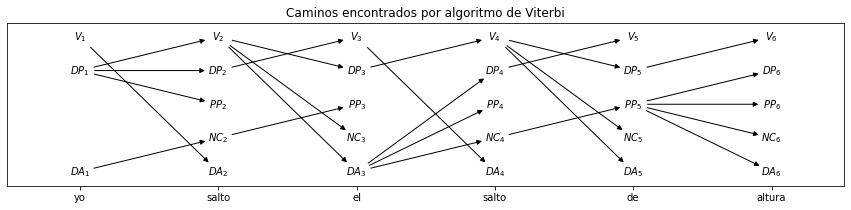
\includegraphics[width=1\textwidth]{hmm/viterbi.png}
    \caption{Gráfica de los caminos después de aplicar el algoritmo de Viterbi}
    \label{Fig:Viterbi}
\end{figure}


\subsection{Ejemplo: etiquetado del lenguaje natural}

Consideremos que queremos etiquetar las categorías gramaticales en lenguaje natural. Esto es, dada una cadena de lenguaje natural, queremos saber cuál es la cadena de etiquetas que le corresponde según las palabras que componen la entrada. Para hacer esto tomaremos algunos símbolos convencionales para etiquetas gramaticales. Estos se muestran en la Tabla~\ref{tab:Tags}.

\begin{table}[]
    \centering
    \begin{tabular}{c c c} \\ \hline
        \textbf{Etiqueta} & \textbf{Descripción} & \textbf{Ejemplo}  \\ \hline
        DA & Determinante Artículo & el, la, los, las \\
        DP & Determinante Pronombre & yo, tú, ella \\
        PP & Preposición & de, ante, para \\
        NC & Nombre Común & gato, perro, flor \\
        V & Verbo & comer, llover, dar \\ \hline
    \end{tabular}
    \caption{Conjunto de etiquetas para etiquetado gramatical}
    \label{tab:Tags}
\end{table}

También podemos tomar palabras del español que correspondan a estas etiquetas, aquí nos limitaremos a algunas de ellas; en particular, usaremos las palabras: `el', `la', `yo', `ellos', `de', 'salto', `altura', `cuerda', `vino', `tomaban' y `saltaban'. Podemos conformar nuestro modelo. Asumiremos que ya hemos estimado las probabilidades.

El vector de iniciales será:

\begin{center}
 \begin{tabular}{l|c}
  \multicolumn{1}{c|}{$y_0$}   &  $P(Y^{(0)})$ \\ \hline
  DA &    0.18 \\
  DP   &    0.5 \\
  PP    &    0.08 \\
  NC & 0.16 \\
  V &  0.08 \\
 \end{tabular}
 \end{center}

 Consideremos la siguiente matriz de probabilidades de transición:

 \begin{center}
 \begin{tabular}{l|ccccc}
  \multicolumn{4}{c}{$P(Y^{(t)}|Y^{(t-1)})$} \\ \hline
  $Y^{(t)}$ \textbackslash $Y^{(t-1)}$          & DA & DP & PP & NC & V \\ \hline
  DA & 0.1  & 0.1  & 0.3 & 0.05 & 0.4 \\
  DP & 0.1  & 0.1  & 0.1 & 0.05 & 0.1 \\
  PP & 0.1  & 0.1  & 0.1 & 0.8  & 0.1 \\
  NC & 0.6  & 0.1  & 0.4 & 0.05 & 0.3 \\
  V  & 0.1  & 0.6  & 0.1 & 0.05 & 0.1 \\
 \end{tabular}
 \end{center}


 Finalmente, la matriz de probabilidades de emisión estará dada como:

\begin{center}
 \begin{tabular}{l|ccccc}
  \multicolumn{4}{c}{$P(Y^{(t)}|Y^{(t-1)})$} \\ \hline
  $Y^{(t)}$ \textbackslash $Y^{(t-1)}$          & DA & DP & PP & NC & V \\ \hline
  el        & 0.23  & 0.05  & 0.05 & 0.01   & 0.05  \\
  la        & 0.23  & 0.05  & 0.05 & 0.01    & 0.05 \\
  yo        & 0.06  & 0.27  & 0.05 & 0.01    & 0.05  \\
  ellos     & 0.06  & 0.28  & 0.05 & 0.05 & 0.05 \\
  de        & 0.06  & 0.05  & 0.55 & 0.05 & 0.05 \\
  salto     & 0.06  & 0.05  & 0.05   & 0.3  & 0.25 \\
  cuerda    & 0.06  & 0.05  & 0.05  & 0.25  & 0.05 \\
  vino      & 0.06  & 0.05  & 0.05   & 0.3  & 0.05 \\
  tomaban   & 0.06  & 0.05  & 0.05   & 0.01    & 0.2 \\
  saltaban  & 0.06  & 0.05  & 0.05   & 0.01    & 0.2 \\
 \end{tabular}
 \end{center}


 Esto define nuestro HMM, por lo que ahora podemos aplicarlo a resolver un problema de etiquetado. Tomemos una cadena simple; sea esta: `ellos tomaban vino'. Procedemos entonces a aplicar el algoritmo de Viterbi. Consideramos que los símbolos de entrada son $x^{(1)} = \text{ellos}$, $x^{(2)} = \text{tomaban}$ y $x^{(3)} = \text{vino}$. Procedemos entonces a realizar el algoritmo:

 \begin{enumerate}
     \item Calculamos los valores $\delta_i(1)$ para los símbolos iniciales, aquí se toma en cuenta el observable $x^{(1)} = ellos$; estos son:
     \begin{align*}
         \delta_{DA}(1) &= 0.06 \cdot 0.18 = 0.01\\
         \delta_{DP}(1) &= 0.28 \cdot 0.5 = 0.14 \\
         \delta_{PP}(1) &= 0.05 \cdot 0.08 = 0.004 \\
         \delta_{NC}(1) &= 0.01 \cdot 0.16 = 0.001 \\
         \delta_{V}(1) &= 0.05 \cdot 0.08 = 0.004\\
     \end{align*}

     \item Ahora generamos los caminos para el siguiente símbolo en la cadena correspondientes a la observación $x^{(2)} = tomaban$:
     %\begin{center}
      %  \small
      %   \begin{tabular}{c c c c c c c} \hline
      %      $\mathbf{\delta}$ & DA & DP & PP & NC & V & $\max$\\ \hline
      %      $\delta_{DA}(2)$  & $0.06\cdot 0.1 \cdot 0.01=0.00006$ & $0.06\cdot 0.1 \cdot 0.14=0.008$ & $0.06\cdot 0.3 \cdot 0.008=0.00014$ & $0.06\cdot 0.05 \cdot 0.008=0.000024$ & $0.06\cdot 0.4 \cdot 0.004=0.00009$ & 0.008 \\
      %      $\delta_{DP}(2)$  & $0.05\cdot 0.1 \cdot 0.01=0.00005$ & $0.05\cdot 0.1 \cdot 0.14=0.0007$ & $0.05\cdot 0.1 \cdot 0.008=0.0004$ & $0.05\cdot 0.05 \cdot 0.008=0.000024$ & $0.05\cdot 0.4 \cdot 0.004=0.00009$ & 0.3 \\
      %   \end{tabular}
     %\end{center}
     \begin{center}
        \small
         \begin{tabular}{c c c c c c | c c} \hline
            $\delta$ & DA & DP & PP & NC & V & $\max$ & $\phi$\\ \hline
            $\delta_{DA}(2)$  & 6.0e-05 & \textbf{8.4e-04} & 7.2e-05 & 3.0e-06 & 9.6e-05 & 8.4e-04 & DP\\
            $\delta_{DP}(2)$  & 5.0e-05 & \textbf{7.0e-04} & 2.0e-05 & 2.5e-06 & 2.0e-05 & 7.0e-04 & DP \\
            $\delta_{PP}(2)$  & 5.e-05 & \textbf{7.e-04} & 2.e-05 & 4.e-05 & 2.e-05 & 7.e-04 & DP \\
            $\delta_{NC}(2)$  & 6.0e-05 &  \textbf{1.4e-04} & 1.6e-05 & 5.0e-07 & 1.2e-05 & 1.4e-04 & DP \\
            $\delta_{V}(2)$  & 2.00e-04 & \textbf{1.68e-02} & 8.00e-05 & 1.00e-05 & 8.00e-05 & 1.68e-02 & DP\\ \hline
         \end{tabular}
     \end{center}

     Observemos que, en este caso, para todas las posibles emisiones en $t=2$, la emisión en el tiempo anterior que produjo la mayor probabilidad fue $DP$.  En general, no necesita ser el caso.

     \item Obtenemos los casos para el último estado correspondientes a la observación $x^{(3)} = vino$:
        \begin{center}
        {\small
         \begin{tabular}{c c c c c c | c c} \hline
            $\delta$ & DA & DP & PP & NC & V & $\max$ & $\phi$\\ \hline
            $\delta_{DA}(3)$  & 5.040e-06 & 4.200e-06 & 1.260e-05 & 4.200e-07 & \textbf{4.032e-04} & 4.032e-04 & V \\
            $\delta_{DP}(3)$  & 4.2e-06 & 3.5e-06 & 3.5e-06 & 3.5e-07 & \textbf{8.4e-05} & 8.4e-05 & V \\
            $\delta_{PP}(3)$  & 4.2e-06 & 3.5e-06 & 3.5e-06 & 5.6e-06 & \textbf{8.4e-05} & 8.4e-05 & V \\
            $\delta_{NC}(3)$  & 1.512e-04 & 2.100e-05 & 8.400e-05 & 2.100e-06 & \textbf{1.512e-03} & \textbf{1.512e-03} & V \\
            $\delta_{V}(3)$  & 4.2e-06 & 2.1e-05 & 3.5e-06 & 3.5e-07 & \textbf{8.4e-05} & 8.4e-05 & V\\ \hline
         \end{tabular}}
     \end{center}
 \end{enumerate}

En este caso todos los caminos son de la forma DP - V. Esto genera un camino, que corresponde a la parte de avance del algoritmo. Ahora tenemos que obtener el retroceso, el cuál nos dará las etiquetas. La última etiqueta corresponderá al camino que tenga mayor probabilidad, que en este caso corresponde a $\delta_{NC}(3)$. Por tanto, la última etiqueta será NC. De aquí recuperaremos los valores de $\phi$ que corresponden al camino, que en este caso es V y DP. Por tanto, las etiquetas finales serán:
$$DP - V - NC$$
Es decir, nuestra cadena `ellos tomaban vino' tiene las etiquetas de pronombre, verbo y nombre común.






\section{Desarrollo}

En esta práctica se implementará el algoritmo de Viterbi para etiquetado de categorías gramaticales de una cadena de lenguaje natural. 
Tómese el HMM del ejemplo anterior, en donde los símbolos de emisiones están dados por: $$Y = \{DA, DP, PP, NC, V\}$$ Y los símbolos de observación se determinan por: $$X = \{el, la, yo, ellos, de, salto, cuerda, vino, tomaban, saltaban\}$$
Utilizamos las probabilidades que se han considerado previamente. El código fuente se puede revisar en el archivo \code{HMMViterbi.ipybn}.

\subsection{Implementación}

Para la implementación del código del algoritmo de Viterbi para el etiquetado de cadenas de lenguaje natural se propone generar la función de avance y de retroceso, para incorporarlas dentro de una función \code{ViterbiParser}. Se sugiere que se utilicen estructuras de datos de arreglos de \code{numpy}, para trabajar con productos de matrices y vectores, que pueden realizar los cálculos de manera más eficiente. La implementación constará de los siguientes elementos:

\begin{itemize}
    \item Se tomará como entrada los parámetros del HMM; las probabilidades pueden representarse por medio de arreglos. Para poder manejarlos adecuadamente, se requiere indexar los símbolos de emisión y observación. Se puede usar una estructura de hash o diccionario para relacionar los símbolos y sus índices. Esta indexación es arbitraria, y sólo debe tomarse en cuenta que debe haber una correspondencia entre los índices y las entradas de los arreglos. 

    \item El método tomará como entrada una cadena del lenguaje natural. Esta cadena debe ser preprocesada. Ya que se están considerando sólo palabras en minúsculas, cualquier cadena debe contener sólo minúsculas y deberán eliminarse símbolos ortográficos en caso de presentarse. Posteriormente, se generarán los tokens, que corresponden a las palabras, separando por espacios en blanco para conformar una lista. Finalmente, se recomienda sustituir los tokens en las cadenas por sus índices numéricos correspondientes.

    \item La inicialización del algoritmo de Viterbi almacena la variable $\delta$ en el tiempo 1, que corresponde al producto de las probabilidades de la observación condicionadas por los iniciales. Esto puede expresarse como el producto punto a punto (que denotamos $\odot$) entre el vector renglón de $B$ correspondiente a la primera observación por el vector de iniciales. Matemáticamente:
    $$\delta(1) \leftarrow B_{x^{(1)}, \cdot} \odot \Pi$$
    Donde $\delta(1)$ es un vector con entradas $\delta_i(1)$ correspondientes a los símbolos. Este producto se expresa en python por el operador \code{x*y}, donde $x$ e $y$ son arreglos.

    \item Para el paso de avance se obtendrán los valores que maximicen los caminos hacia la emisión en el estado actual. Esto se obtiene para todas las emisiones. Ya que se debe computar los valores $B_{x^{t+}, i} \delta_k(t)$ se puede tomar un producto externo, para generar una matriz que contenga estos productos y posteriormente se multiplique por la matriz de transición $A$. Finalmente, se obtendrán los valores máximos sobre los renglones de la matriz resultante. Se recomienda usar una variable $p$ que contenga sólo las probabilidades; esta variable se computará entonces como:
    $$p\leftarrow A \odot \Big( B_{x^{(t+1)}, \cdot} \otimes \delta(t) \Big)$$
    Aquí $\otimes$ representa el producto externo, el cual se expresa en python por medio de la paquetería numpy como \code{numpy.outer()}.  De esta forma se pueden obtener tanto los valores para la variable $\delta$ (valores máximos) como para la variable $\phi$ (las etiquetas o argumentos que maximizan las probabilidades. La variable $\phi$ guardará las emisiones que terminarán etiquetando a la cadena. Los máximos y los mínimos pueden obtenerse con los métodos \code{numpy.max()} y \code{numpy.argmax()}.

    \item Una vez concluido el paso de avance, el paso de retroceso comenzará generando la última etiqueta; es decir, la etiqueta que corresponde a la última palabra de la cadena de entrada y posteriormente avanzará hacia atrás sobre las variables $\phi$ para generar la cadena de etiquetas de emisión. Para concluir se revertirá la cadena para obtener las etiquetas en el orden correcto. Si se ha trabajado con índices numéricos, se recuperarán las etiquetas correspondientes a este índice.
    \item El etiquetador en base a HMMs y Viterbi se probará sobre diferentes cadenas del lenguaje que contengan las palabras en las observaciones. Se sugiere probar en la cadena `yo salto el salto de altura', donde se puede comprobar la calidad del etiquetado. 
\end{itemize}


\section{Requisitos y resultados}

El sistema de etiquetado deberá ser una función que pueda trabajar con cualquier cadena que contenga los tokens (palabras) consideradas en las observaciones. En caso de observar un token que no está se podrá ignorar o emitir un mensaje de error. Se espera que la salida sea una cadena con las etiquetas correspondientes a las categorías gramaticales de los tokens en la entrada. El código deberá estar adecuadamente comentado. Se tomarán en cuenta los siguientes resultados.

\begin{enumerate}
 \item Que el manejo de las cadenas de lenguaje natural y etiquetas de emisión sea adecuado.
 \item Que la representación de los datos se maneje adecuadamente; en particular, que las operaciones para el algoritmo de Viterbi entre las matrices y los vectores sean eficientes.
 \item Que tanto la entrada como la salida sean cadenas interpretables por el usuario humano.
\end{enumerate}
